\section{A Precise Full-Wave Rectifier: pt.II}

\subsection{Experiment Design}
    \subsubsection{Background}
        In the last chapter, we constructed a precise Full-Wave Rectifier using two Op.Amp. as core components. In this chapter, we will construct another type of precise full-wave rectifier also with two Op.Amp. and diodes.\par

    \subsubsection{Propose}
    \begin{itemize}
        \item Tested another full-wave rectifier circuit
    \end{itemize}

\subsection{Experiment Design}
    \subsubsection{Materials}
        In this experiment, we will use the following components:
        \begin{itemize}
            \item 1N4148 Diode
            \item LM741 Op.Amp.
            \item Resistors
            \item Breadboard
            \item DC power supply
            \item Digital Multi-Meter
            \item Function Generator
            \item Oscilloscope
        \end{itemize}

    \subsubsection{Circuit Diagram}
        The following circuit diagrams 
        \begin{figure}[H]
            \centering
                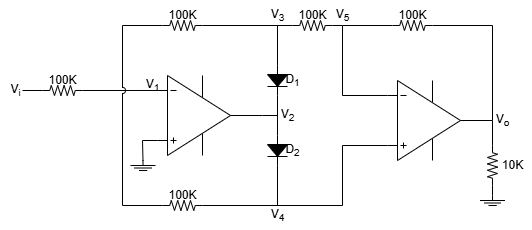
\includegraphics[width=0.7\linewidth]{Experiment_14/Circuit/Lab14.drawio.png}
                \caption{Full-Wave Rectifier Circuit II}
                \label{cir:14}
        \end{figure}

    \subsubsection{Theoretical Analysis}
        \begin{enumerate}[a]
            \item \textbf{}
        \end{enumerate}

\subsection{Experiment record}
    \subsubsection{AC Analysis}
    The output waveform with $V_i$ with input sinusoidal signal with a frequency 200 Hz:\par
    \begin{figure}[H]
        \centering
        \begin{subfigure}{0.3\linewidth}
            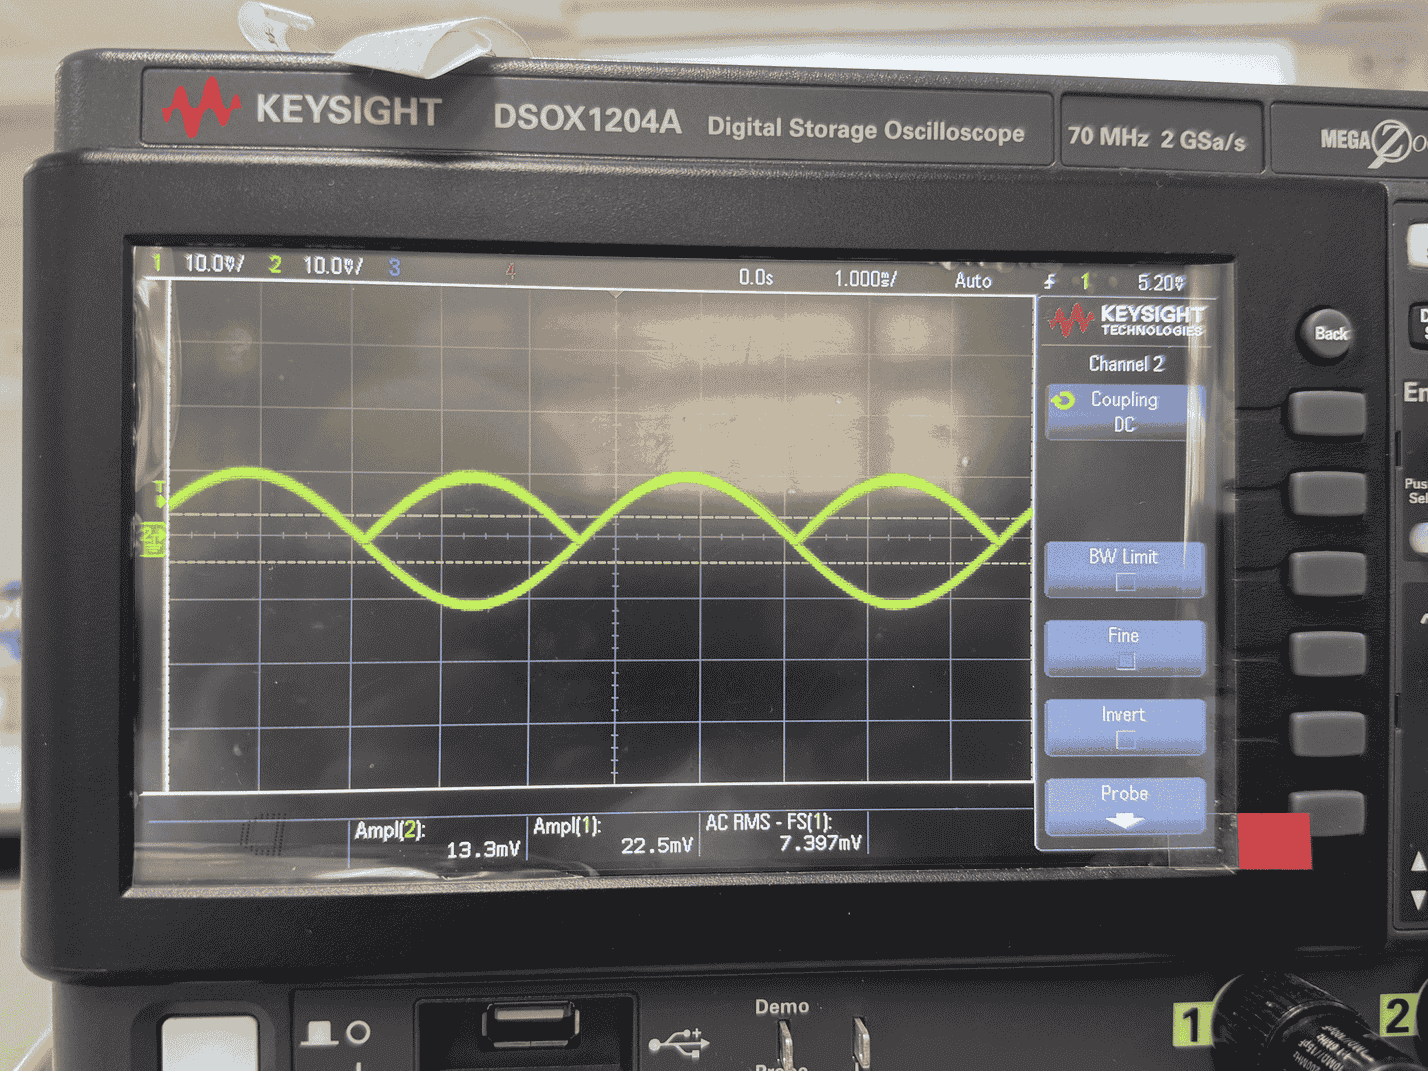
\includegraphics[width=1\linewidth]{Experiment_14/Images/lab14_0-1v.png}
            \caption{Amplitude $v_i=0.1V$}
            \label{wave:14-AC0}
        \end{subfigure}
        \begin{subfigure}{0.3\linewidth}
            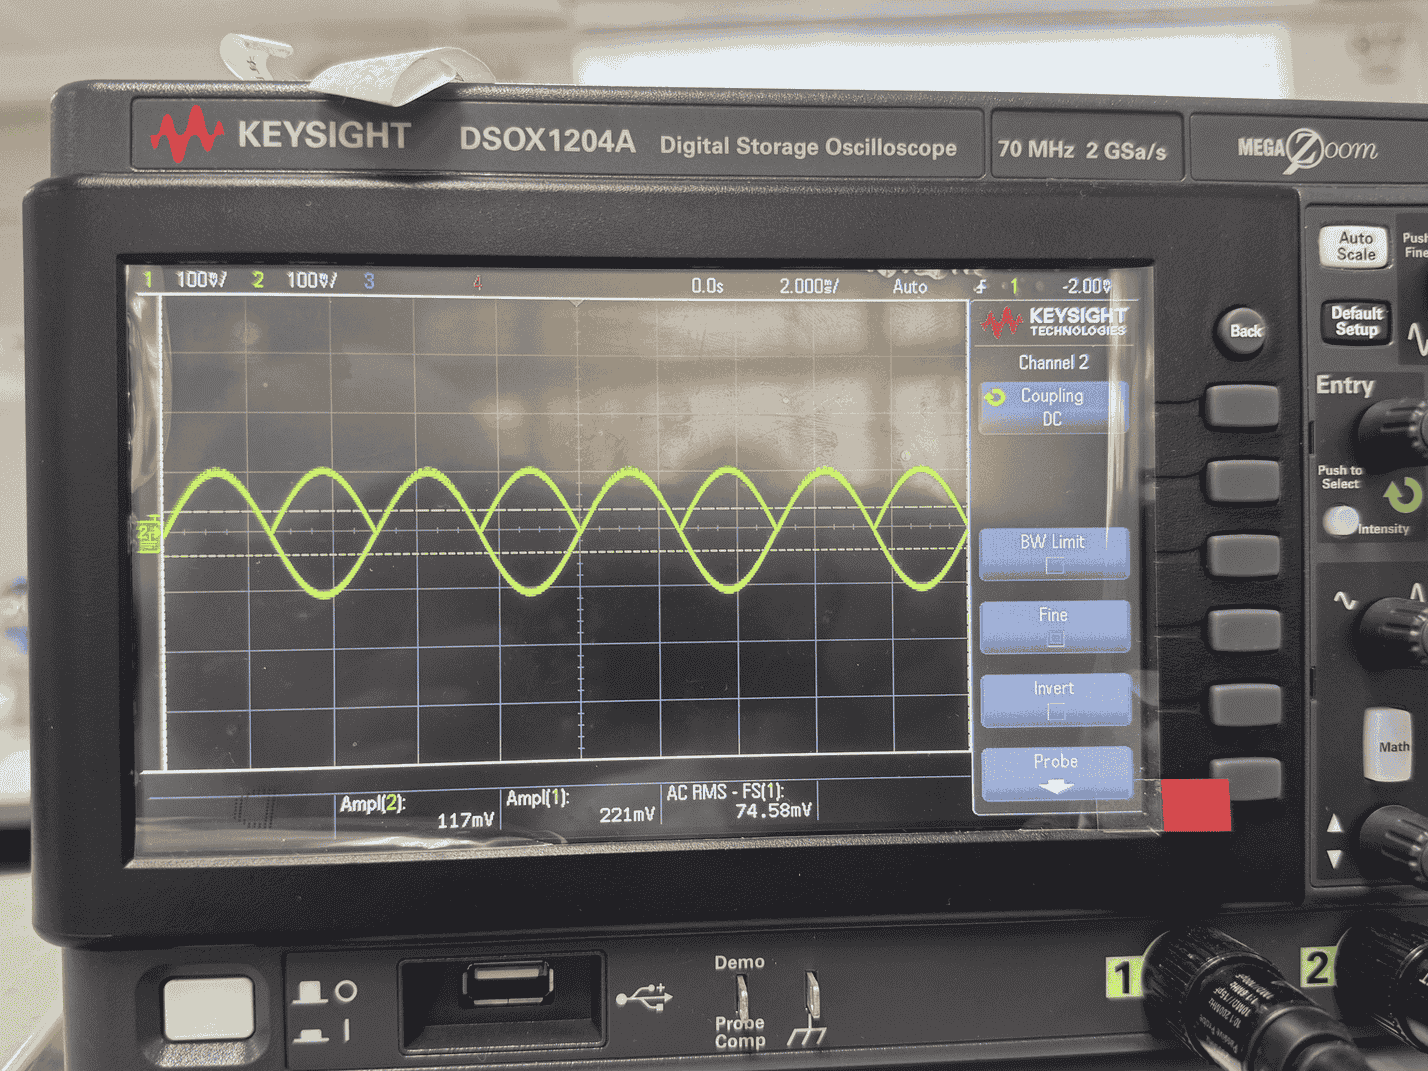
\includegraphics[width=1\linewidth]{Experiment_14/Images/lab14_1v.png}
            \caption{Amplitude $v_i=1V$}
            \label{wave:14-AC1}
        \end{subfigure}
        \begin{subfigure}{0.3\linewidth}
            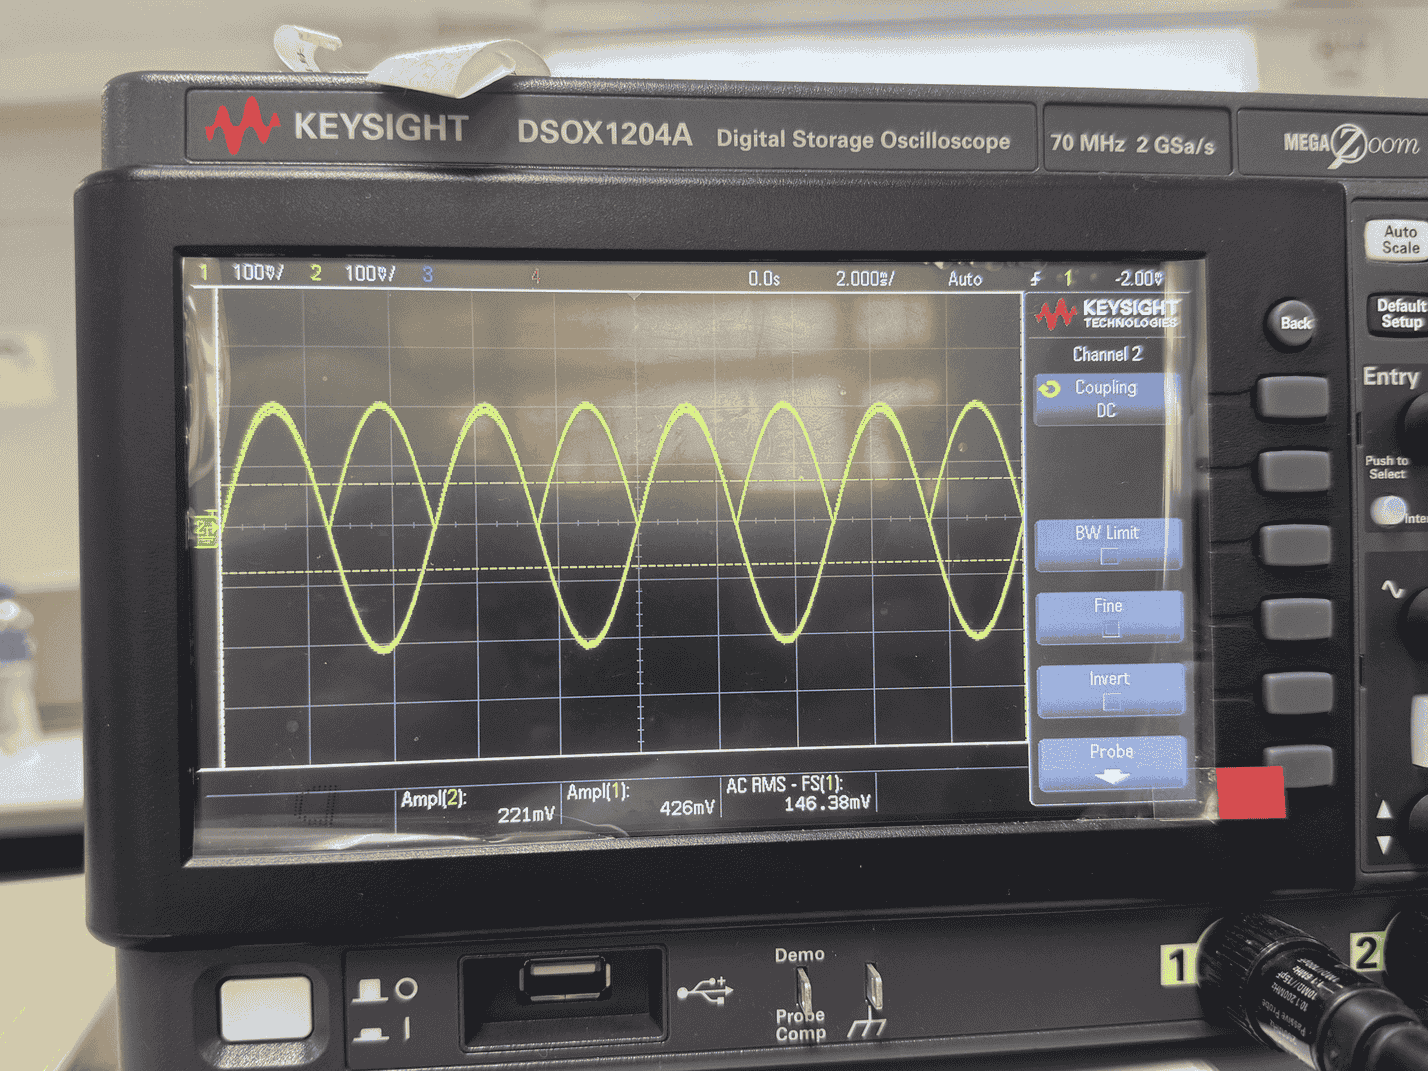
\includegraphics[width=1\linewidth]{Experiment_14/Images/lab14_2v.png}
            \caption{Amplitude $v_i=2V$}
            \label{wave:14-AC2}
        \end{subfigure}

        \begin{subfigure}{0.3\linewidth}
            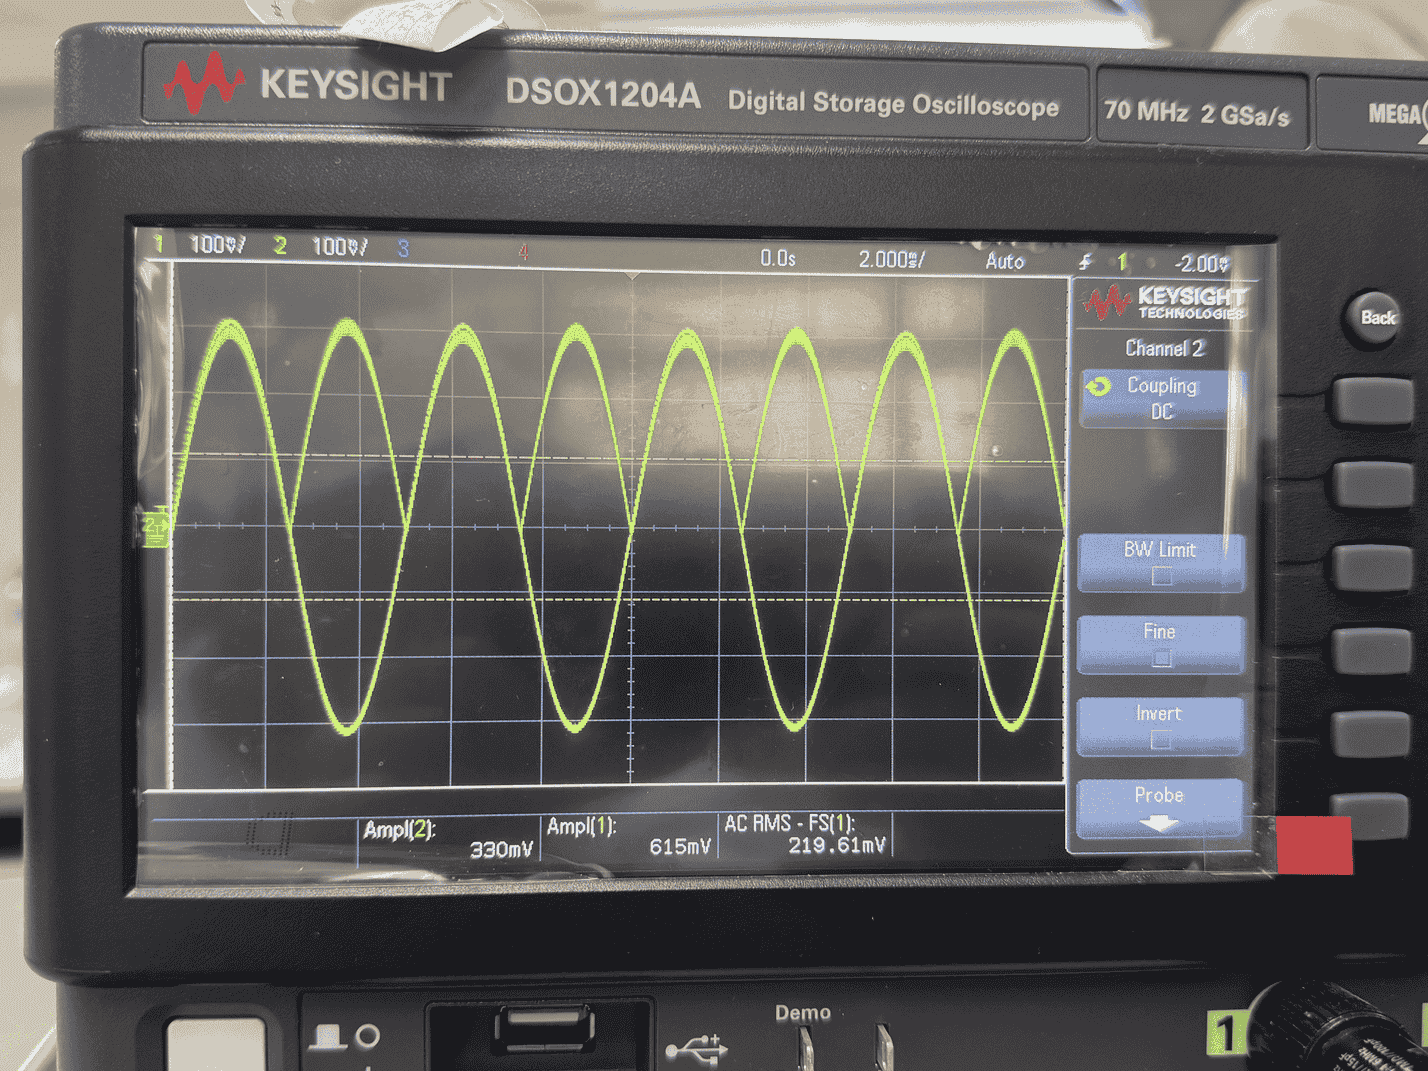
\includegraphics[width=1\linewidth]{Experiment_14/Images/lab14_3v.png}
            \caption{Amplitude $v_i=3V$}
            \label{wave:14-AC3}
        \end{subfigure}
        \begin{subfigure}{0.3\linewidth}
            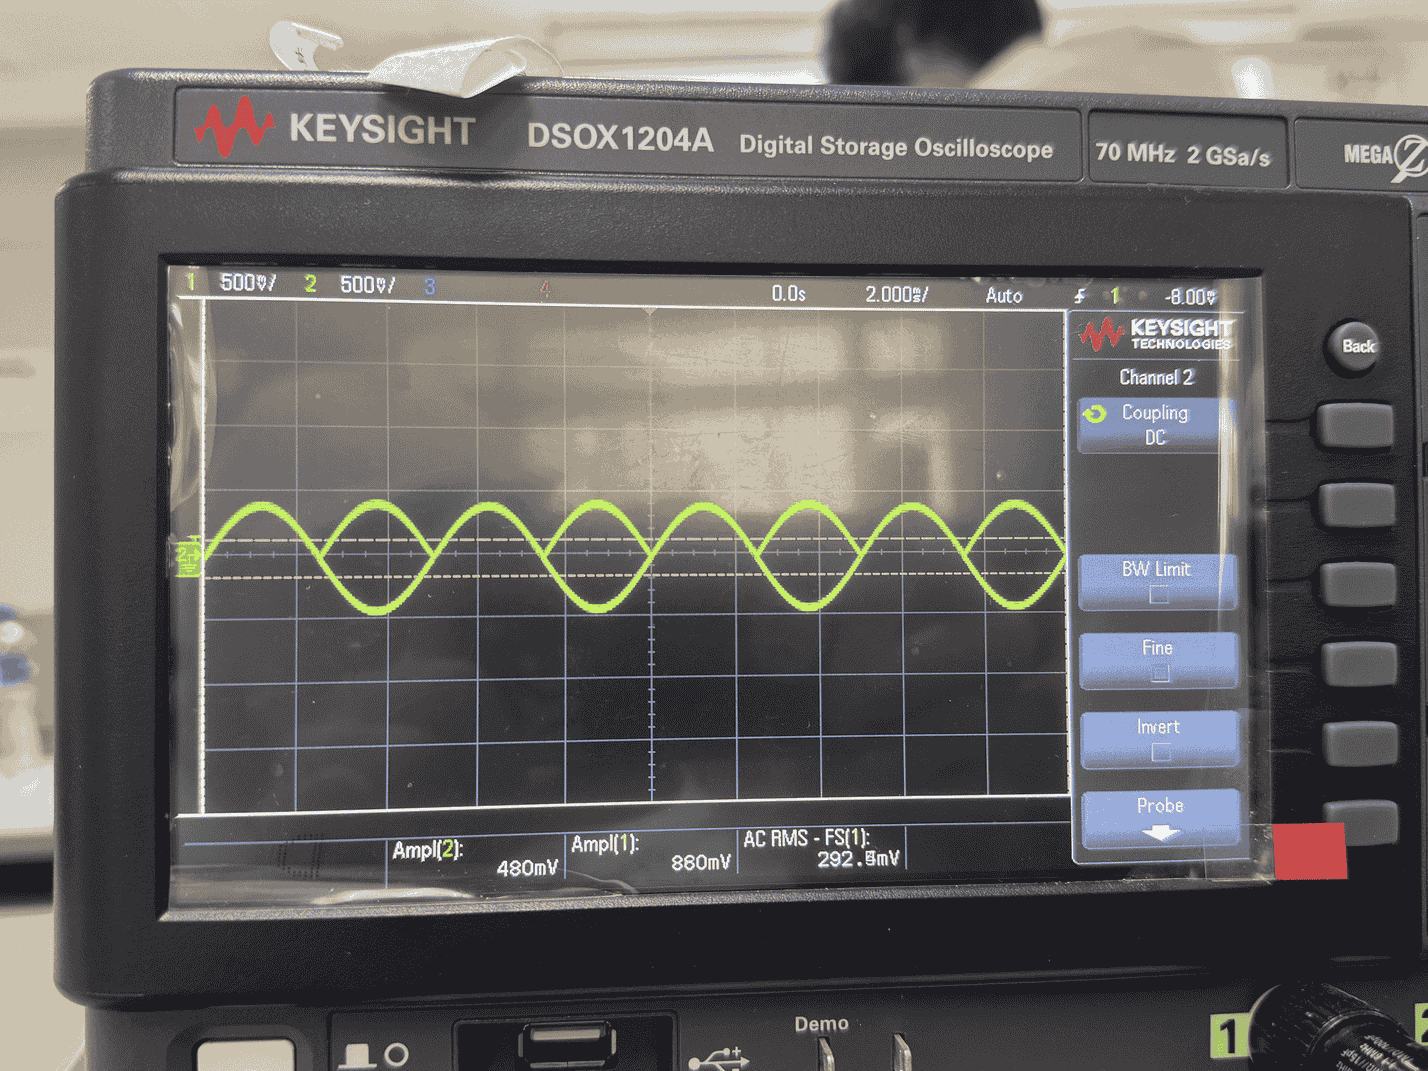
\includegraphics[width=1\linewidth]{Experiment_14/Images/lab14_4v.png}
            \caption{Amplitude $v_i=4V$}
            \label{wave:14-AC4}
        \end{subfigure}
        \begin{subfigure}{0.3\linewidth}
            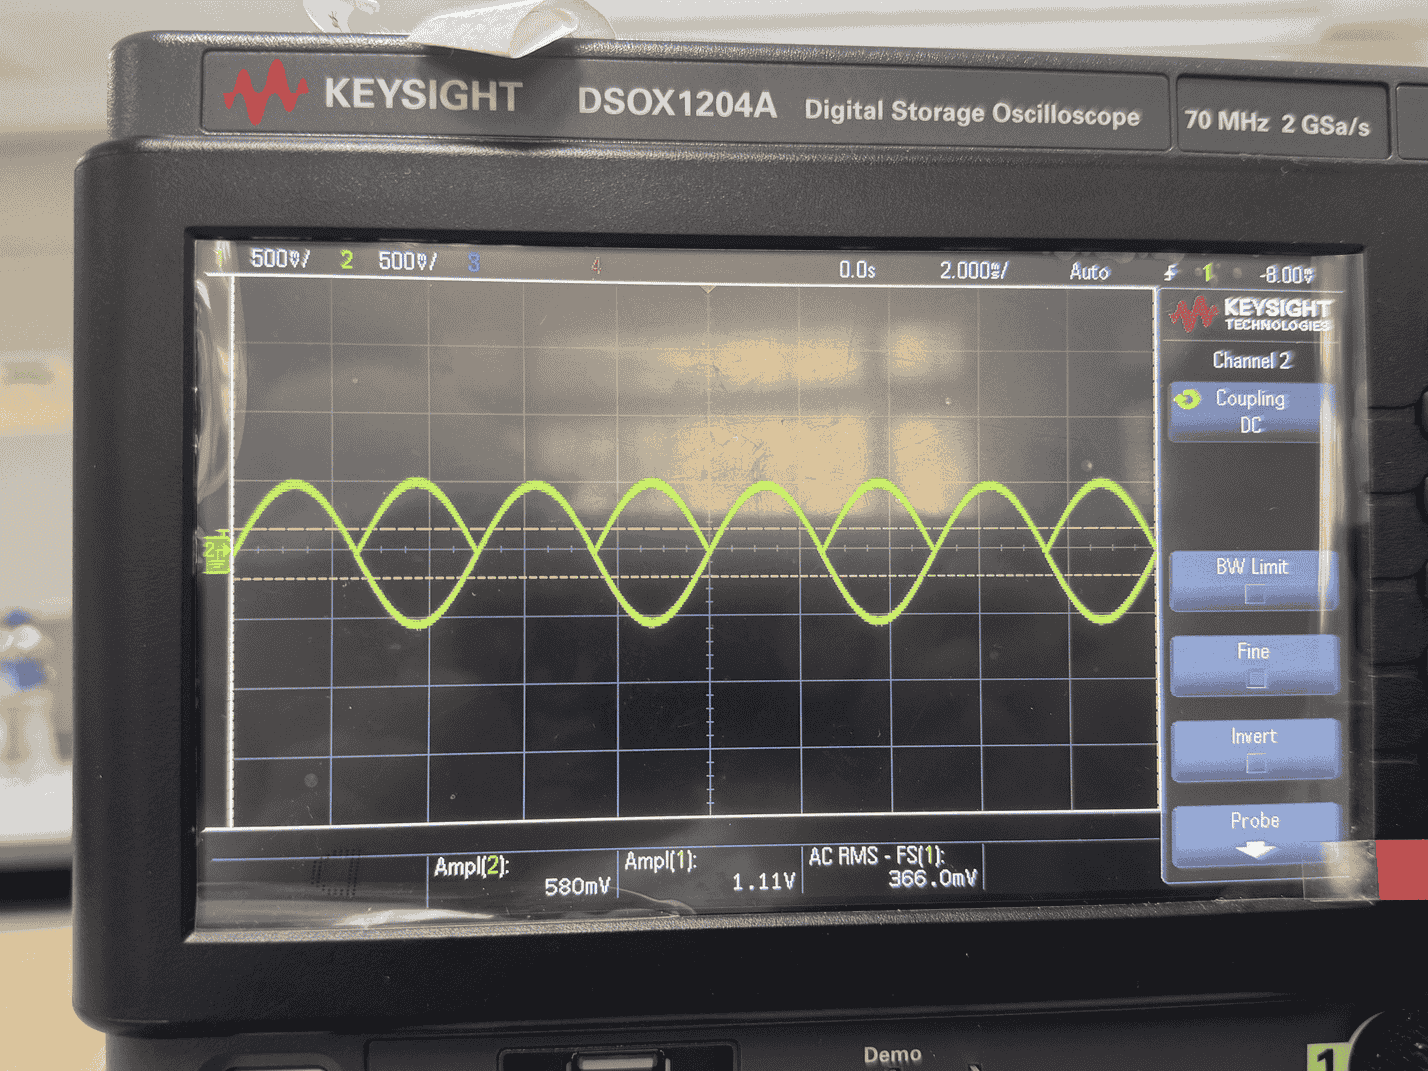
\includegraphics[width=1\linewidth]{Experiment_14/Images/lab14_5v.png}
            \caption{Amplitude $v_i=5V$}
            \label{wave:14-AC5}
        \end{subfigure}


        \caption{Output Waveform of Full-Wave Rectifier Circuit II}
    \end{figure}
    \FloatBarrier

    \subsubsection{DC Analysis}
        For DC analysis, we change the input into a DC signal source, and vary the voltage $V_i$ from -12V to 12V, and record the output voltage $V_o$ and the voltage of each node $V_1$ to $V_5$. The recorded data is shown in the following table:
    \begin{table}[H]
        \centering
    \begin{tabular}{l|rrrrrr}
        $V_i$  & -12   & -5    & -1    & 1     & 5     & 12 \\
        \midrule
        $V_1$   & -0.408 & 0     & 0     & 0     & 0     & 1.562 \\
        $V_2$   & 8.68  & 3.799 & 1.03  & -1.42 & -5.504 & -9.4 \\
        $V_3$   & 2.548 & 1.64  & 0.32  & -1    & -5    & -8.875 \\
        $V_4$   & 8.195 & 3.353 & 0.66  & 0     & 0     & 1.549 \\
        $V_5$   & 5.617 & 3.353 & 0.66  & 0     & 0     & 0.0585 \\
        $V_o$   & 8.61  & 4.983 & 0.99  & 0.959 & 4.795 & 8.6 \\
        \end{tabular}%
        \caption{Node voltages collected with Circuit II}
    \end{table}
\subsection{Experiment Conclusion}
    \subsubsection{Conclusion}
    In this experiment, we have constructed and tested a full-wave rectifier circuit. We have observed the output waveform with different input voltages and frequencies.